%%%%%%%%%%%%%%%%%%%%%%%%%%%%%%%%%%%%%%%%%
% Short Sectioned Assignment
% LaTeX Template
% Version 1.0 (5/5/12)
%
% This template has been downloaded from:
% http://www.LaTeXTemplates.com
%
% Original author:
% Frits Wenneker (http://www.howtotex.com)
%
% License:
% CC BY-NC-SA 3.0 (http://creativecommons.org/licenses/by-nc-sa/3.0/)
%
%%%%%%%%%%%%%%%%%%%%%%%%%%%%%%%%%%%%%%%%%

%----------------------------------------------------------------------------------------
%	PACKAGES AND OTHER DOCUMENT CONFIGURATIONS
%----------------------------------------------------------------------------------------
\documentclass[11pt]{article}
\usepackage{geometry} % Pour passer au format A4
\geometry{hmargin=1cm, vmargin=1cm} % 


\usepackage[T1]{fontenc} % Use 8-bit encoding that has 256 glyphs
\usepackage[english,francais]{babel} % Français et anglais
\usepackage[utf8]{inputenc} 

\usepackage{amsmath,amsfonts,amsthm} % Math packages

\usepackage{lmodern}
\usepackage{url}
\usepackage{eurosym} % signe Euros
\usepackage{geometry} % Pour passer au format A4
\geometry{a4paper} % 
\usepackage{graphicx} % Required for including pictures
\usepackage{float} % Allows putting an [H] in \begin{figure} to specify the exact location of the figure

\usepackage{multicol}
\usepackage{sectsty} % Allows customizing section commands
\allsectionsfont{\centering \normalfont\scshape} % Make all sections centered, the default font and small caps

%----------------------------------------------------------------------------------------
%	Pied de Page
%----------------------------------------------------------------------------------------

\setlength\parindent{0pt} % Removes all indentation from paragraphs - comment this line for an assignment with lots of text


%----------------------------------------------------------------------------------------
%	Titre
%----------------------------------------------------------------------------------------

\newcommand{\horrule}[1]{\rule{\linewidth}{#1}} % Create horizontal rule command with 1 argument of height


%----------------------------------------------------------------------------------------
%	Début du document
%----------------------------------------------------------------------------------------

\title{Symétrie Centrale} % Title
\author{$5^e 1$}
\date{26 Septembre 2013} % Date for the report
\begin{document}

\maketitle % Insert the title, author and date

%\begin{center}
%\textsf{--}\\
%\textsf{La réalité, c'est ce qui refuse de disparaître quand on cesse d'y croire.}\\
%\texttt{Philip K. Dick}\\
%\textsf{--}
%\end{center}
%----------------------------------------------------------------------------------------
%	SECTION 1
%----------------------------------------------------------------------------------------
\thispagestyle{empty}
\textbf{Exo 1 : À l'aide du quadrillage}

\begin{figure}[H]
  \centering
  \includegraphics[width=0.8\linewidth]{sources/exo/sym-cen-1.pdf}
  \label{fig:exo1}
\end{figure}

\begin{enumerate}
\item Trouver $A_1$, $B_1$, $C_1$, $D_1$, $E_1$ les symétriques de $A$, $B$, $C$, $D$, $E$ par rapport à $O_1$.
\item Relier E avec D avec C avec B avec A. Faire de même pour la figure 1.
\item Trouver$A_2$, ..., $E_2$ les symétriques de $A$, ..., $E$ par rapport à $O_2$ et relier les points.
\item Tracer les droites (jusqu'au cadre) (AB), ($A_1, B_1$) et ($A_2, B_2$). En déduire une propriété sur le symétrique d'une droite.
\end{enumerate}

\textbf{Exo 2 : Avec une règle et un compas}

\begin{figure}[H]
  \centering
  \includegraphics[width=0.8\linewidth]{sources/exo/sym-cen-2.pdf}
  \label{fig:exo2}
\end{figure}
\begin{enumerate}
\item Trouver $A_1$, $B_1$, $C_1$, $D_1$ les symétriques de $A$, $B$, $C$, $D$ par rapport à $O_1$.
\item Reproduire la figure avec les points précédement trouvés.
\item Faire de même avec $A_2$, $B_2$, $C_2$, $D_2$ et $E_2$ les symétriques de $A$, $B$, $C$, $D$ et $E$ par rapport à $O_2$. Tracer la figure pour les points de la figure 2.
\item En déduire une propriété sur le symétrique d'un cercle.
\end{enumerate}

%------------------------------------------------
\section{Exercices}
%------------------------------------------------

%-----------------------------------111111111111111111111111111111
\subsection{Tracer des symétriques}
%-----------------------------------------------------------------

\subsubsection{Correction}

\textbf{Exemple de cours}

\begin{figure}[H]
  \centering
  \includegraphics[width=0.8\linewidth]{sources/exo/sym-cen-1-cor.pdf}
  \label{fig:exo2}
\end{figure}

\begin{figure}[H]
  \centering
  \includegraphics[width=0.8\linewidth]{sources/exo/sym-cen-2-cor.pdf}
  \label{fig:exo2}
\end{figure}


\textbf{18 - p178}\\

\subsection{rendre une figure symétrique}

\textbf{18 - p178}\\

\subsection{Trouver le symétrique}

\textbf{70 - p187}\\

\subsection{Travaux de recherche}

\begin{enumerate}
\item \textbf{Yin et Yang}
  Éffectuer un travail de recherche et d'ouverture sur le sujet du Yin et du Yang.\\
  Rèf : http://fr.wikipedia.org/wiki/Yin\_et\_yang\\

  \begin{figure}[H]
    \centering
    \includegraphics[width=.6\linewidth]{sources/exo/re_yin_yang.pdf}
    \label{fig:ch2-yy}
  \end{figure}
  
\item \textbf{Maurits Cornelis Escher}\\
  Rechercher une œuvre de M.C. Escher comportant une symétrie centrale.
  
  \begin{figure}[H]
    \centering
    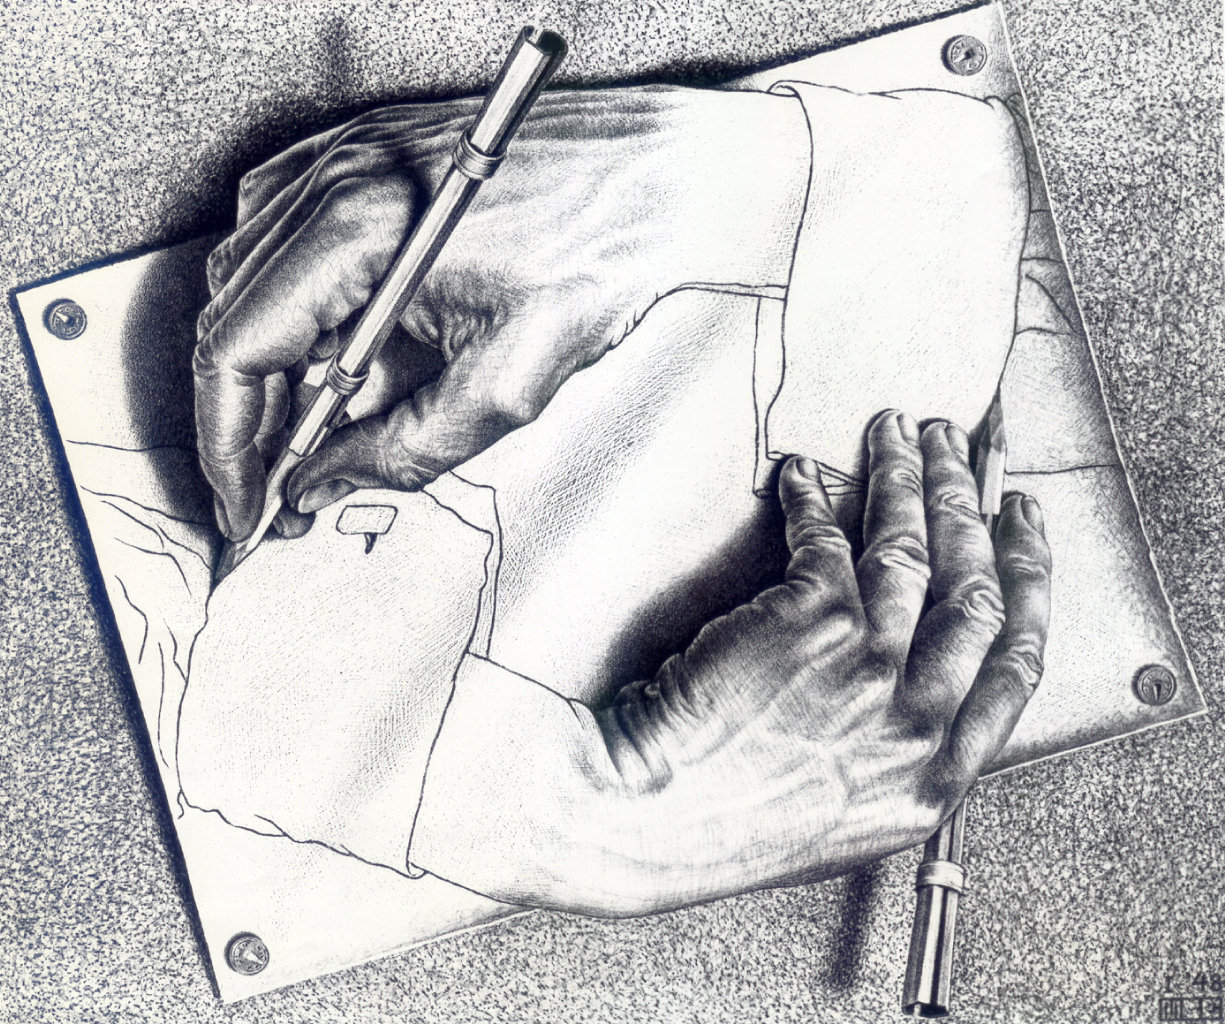
\includegraphics[width=.6\linewidth]{sources/exo/re_escher.jpg}
    \caption{Drawing Hands  - M.C. Escher - 1948 - usage loyal}
    \label{fig:ch2-escher}
  \end{figure}
  Cette exemple n'est pas une symétrie centrale parfaite car il y est représenté une main gauche et une main droite. Néanmoins, elle en est une très belle représentation.\\
  
  Exemples données et présentées : 
  \begin{itemize}
  \item Drawing Hands, 1948
  \item Division 1956 woodcut
  \item Smaller abd Smaller, 1956
  \item Circle Limit II, 1959
  \item The triangle tessellation of the Poincaré, 
  \end{itemize}
  
\end{enumerate}


\end{document}
